\documentclass[11pt]{article}

% colors
\usepackage[table]{xcolor}
\definecolor{maroon}{RGB}{153,0,18}
\definecolor{lime}{RGB}{190,213,88}
\definecolor{sand}{RGB}{217,202,179}
\definecolor{fire}{RGB}{144,50,61}
\definecolor{brick}{RGB}{94,11,21}
\definecolor{olive}{RGB}{117,109,84}
\definecolor{lavpink}{RGB}{172,123,132}
\definecolor{darkpurp}{RGB}{49,10,49}
\definecolor{salmon}{RGB}{204,90,113}
\definecolor{mauve}{RGB}{94,73,85}
\definecolor{greyblue}{RGB}{125,132,145}
\definecolor{greypurp}{RGB}{68,56,80}
\definecolor{brightpurp}{RGB}{96,20,255}

% packages (please add in alphabetical order)
\usepackage{adjustbox}
\usepackage{amsfonts}
\usepackage{amsmath}
\usepackage{amssymb}
\usepackage{array}
\usepackage{bm}
\usepackage{booktabs}
\usepackage{caption}
\usepackage{epstopdf}
\usepackage{float}
\usepackage[margin=1in]{geometry}
\usepackage{graphicx}
\usepackage[colorlinks=true, linkcolor=brightpurp, citecolor=brightpurp, urlcolor=salmon]{hyperref}
\usepackage{lipsum}
\usepackage{longtable}
\usepackage{mathtools}
\usepackage{multirow}
\usepackage{natbib}
\usepackage{rotating}
\usepackage{setspace}
\usepackage{subcaption}
%\usepackage{threeparttable}
\usepackage{threeparttablex}
\usepackage{xr}
\usepackage[printwatermark]{xwatermark}


\newcolumntype{L}[1]{>{\raggedright\let\newline\\\arraybackslash\hspace{0pt}}m{#1}}
\newcolumntype{C}[1]{>{\centering\let\newline\\\arraybackslash\hspace{0pt}}m{#1}}
\newcolumntype{R}[1]{>{\raggedleft\let\newline\\\arraybackslash\hspace{0pt}}m{#1}}

% commands
\newcommand{\mr}{\multirow}
\newcommand{\mc}{\multicolumn}


\begin{document}

\begin{sidewaysfigure}[H]
\centering
\caption{Labor Income Profiles}\label{fig:control-sub}
\begin{subfigure}[h]{0.4\textwidth}
		\centering
		\caption{Forecasted for ABC/CARE Males} \label{fig:abcare1}
		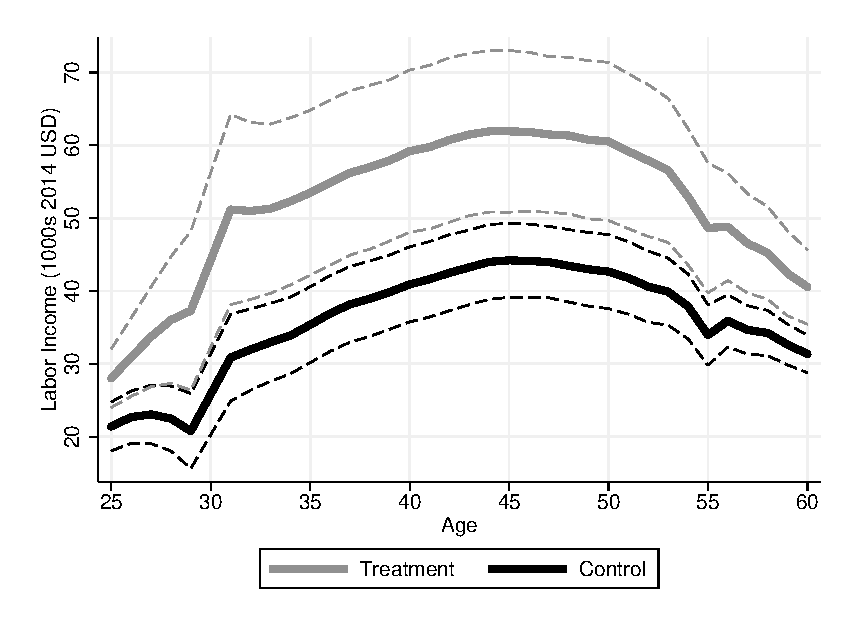
\includegraphics[width=\textwidth]{output/labor_25-60_male.eps}
\end{subfigure}%
\begin{subfigure}[h]{0.4\textwidth}
	\centering
	\caption{PSID, Disadvantaged Males} \label{fig:psid1}
		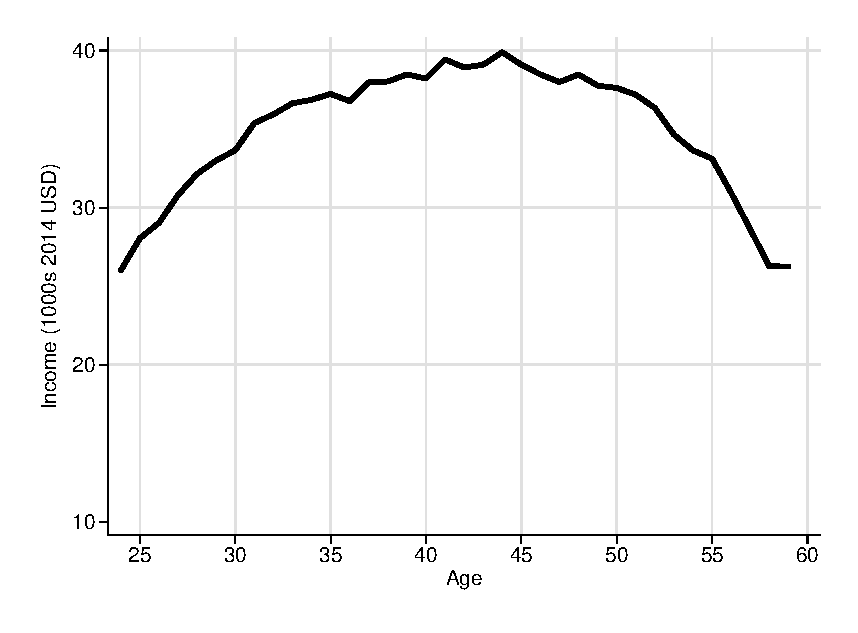
\includegraphics[width=\textwidth]{output/psid_incomeprofiles_s1.eps}
\end{subfigure}

\begin{subfigure}[h]{0.4\textwidth}
		\centering
		\caption{Forecasted for ABC/CARE Females} \label{fig:abcare0}
		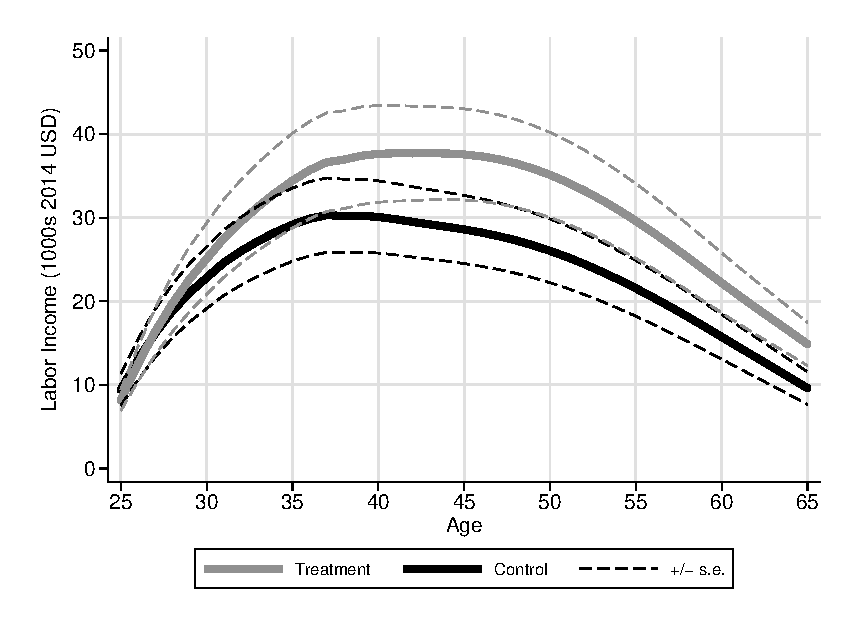
\includegraphics[width=\textwidth]{output/labor_25-60_female.eps}
\end{subfigure}%
\begin{subfigure}[h]{0.4\textwidth}
	\centering
	\caption{PSID, Disadvantaged Females} \label{fig:psid0}
		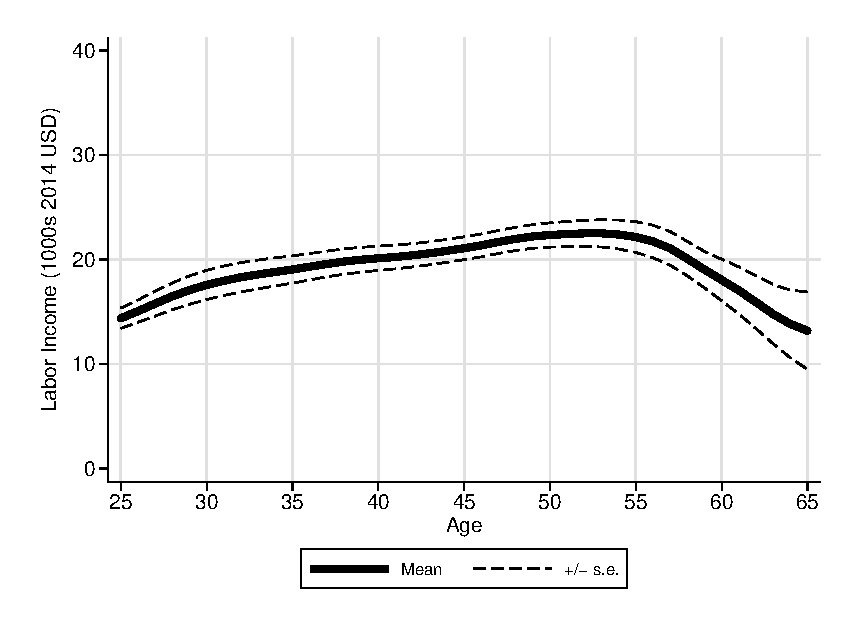
\includegraphics[width=\textwidth]{output/psid_incomeprofiles_s0.eps}
\end{subfigure}
\footnotesize \justify
Note: Panels (a) and (c) display the forecasted labor income profiles for ABC/CARE males and females by treatment status, based on forecasts that combine data from the Panel Study of Income Dynamics (PSID), the National Longitudinal Survey of Youth 1979 (NLSY79), and the Children of the National Longitudinal Survey of Youth 1979 (cNLSY79). Panels (b) and (d) display the median labor income profile of disadvantaged males females in the Panel Study of Income Dynamics (PSID), where disadvantaged is defined as having 12 years of education or less.
\end{sidewaysfigure}

\end{document}